\documentclass{standalone}

\usepackage{tikz}

\usetikzlibrary{positioning, chains, shapes.geometric, fit, shapes, arrows.meta, calc}

\begin{document}

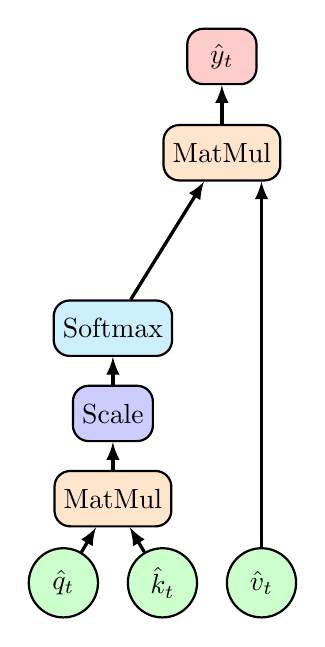
\begin{tikzpicture}[
    >=LaTeX,
    % Styles
    layer/.style={
        rectangle,
        fill=white!10,
        rounded corners=2mm,
        minimum height=2em,
        minimum width=3em,
        draw,
        thick
    },
    arrow/.style={
        -latex,
        very thick
    },
    cell/.style={
        rectangle,
        fill=white!10,
        rounded corners=2mm,
        minimum height=2em,
        minimum width=2.5em,
        draw,
        thick
    },
    input/.style={
        circle,
        fill=green!20,
        rounded corners=2mm,
        minimum height=2em,
        minimum width=2.5em,
        draw,
        thick
    },
    scale_layer/.style={
        rectangle,
        fill=blue!20,
        rounded corners=2mm,
        minimum height=2em,
        minimum width=2.5em,
        draw,
        thick
    },
    matmul/.style={
        rectangle,
        fill=orange!20,
        rounded corners=2mm,
        minimum height=2em,
        minimum width=2.5em,
        draw,
        thick
    },
    output/.style={
        rectangle,
        fill=red!20,
        rounded corners=2mm,
        minimum height=2em,
        minimum width=2.5em,
        draw,
        thick
    },
    softmax/.style={
        rectangle,
        fill=cyan!20,
        rounded corners=2mm,
        minimum height=2em,
        minimum width=2.5em,
        draw,
        thick
    },
    arrow/.style={
        -latex,
        very thick
    }
]

    % Layers
    \node[input] (Q) {$\hat{q}_t$};
    \node[input, right=1em of Q] (K) {$\hat{k}_t$};
    \node[input, right=1em of K] (V) {$\hat{v}_t$};

    \node[matmul, above=2em of $(Q)!0.5!(K)$] (matmul) {MatMul};
    \node[scale_layer, above=1em of matmul] (scale) {Scale};
    \node[softmax, above=1em of scale] (softmax) {Softmax};
    \node[matmul, above=14.5em of $(Q)!0.8!(V)$] (matmul2) {MatMul};
    \node[output,above=1.4em of matmul2] (result) {$\hat{y}_t$};

    % Paths
    \draw[arrow] (Q) -- (matmul);
    \draw[arrow] (K) -- (matmul);
    \draw[arrow] (matmul) -- (scale);
    \draw[arrow] (scale) -- (softmax);
    \draw[arrow] (softmax) -- (matmul2);
    \draw[arrow] (matmul2) -- (result);
    \path[draw, arrow] (V) -- ++(0, 14.5em);
\end{tikzpicture}

\end{document}